\section{Further application results}\label{supp:app-more}

\subsection{Reconstructing the cell-week table}\label{sec:app-data}

The table built by the original pipeline has 70{,}033{,}444 rows but only 34{,}671{,}180
distinct cell-weeks (Section~\ref{sec:data-acled}). In one partition, 613{,}459
cell-weeks appear once, while others appear 2, 3, 8, 16, 32, 48 and up to 648 times.
The national indicators and IPC regions are attached by spatial intersection and then
merged on cell and year. A cell that touches several countries or IPC regions is
therefore multiplied at every join, and each copy combines indicators from different
units.

The duplication matters for more than the covariates. The four-week event counts of
the original pipeline are computed row by row within each cell, after sorting by cell
and week. When a cell-week has copies, the rows immediately before a given row are
copies of the same week, so the ``past'' count contains the current week's events,
which are the outcome. We recomputed the original counts exactly and compared them
with the true counts over the four previous weeks, on 69.4 million rows of the
duplicated table, over all years and without the coverage filter. Among rows with an
event, counting each copy separately, 22\% have an original count that includes the
current week's events while the true past count is zero, for both outcomes. Used
directly as a predictor of the outcome on these rows, without any model, the original
count reaches an AUC-PR of 0.883 for conflict and 0.833 for unrest. The true count
reaches 0.495 and 0.450. These values describe the duplicated table as a whole. They
are not on the same rows as the test-period scores below. The leak arises only in
cell-weeks that have copies, and never in the first copy of a cell-week, which is the
one the repaired table keeps. Copies come from cells that intersect several countries
or several IPC regions; we have not checked how many of them lie on international
borders.

The repaired table has one row per cell-week (Section~\ref{sec:data-acled}). After
ACLED coverage and the biome exclusion it has 19{,}364{,}639 cell-weeks in
59{,}339 cells and 366 weeks. The test period has 4{,}787{,}224 cell-weeks in 46{,}031
cells with complete climate records.

\subsection{Joint prediction when both outcomes are observed}\label{supp:app-jointpred}

When both outcomes are observed in the same places, the joint model cannot be expected
to forecast either one better than univariate models that use both histories as
covariates (Section~\ref{sec:sim-holdout}), and it does not.

\paragraph{Prediction.} All predictive probabilities below are posterior means of
$\operatorname{expit}(\eta)$ over the same 200 posterior draws for every model. The joint model does not
forecast either outcome alone better. Its test log score for conflict is 0.1021,
against 0.1016 for the univariate static model and 0.1017 for the univariate
space-time model (AUC-PR 0.464, 0.470 and 0.470, at a conflict prevalence of 4.2\%),
and for unrest 0.0481 against 0.0481 and 0.0482. In the test period both events occur
in 0.35\% of the 260{,}520 cell-weeks, and conflict occurs in 25.1\% of cell-weeks
with unrest against 3.9\% of those without. Even so, the joint model does not predict the two
outcomes together better than the product of the univariate models. Its joint log score is 0.14993, against 0.14991 for the
product of the univariate space-time models (difference $+0.00003$, SE $0.0005$
clustered by country) and 0.14978 for the product of the univariate static models
($+0.0002$, SE $0.0006$). Within the joint model, drawing the two outcomes jointly
rather than independently improves the joint log score by $0.0002$ (SE $0.0001$), and
conditioning on same-week unrest improves the log score of conflict from 0.1021 to
0.1019 (AUC-PR 0.464 to 0.466). These are small effects. The dependence between the
outcomes in a cell-week is largely carried by the histories and the static effects,
which the univariate models also contain, and the shared field adds little to it at the
weekly scale. As in S5, prediction cannot decide between escalation and shared episodes. The joint fit took about 4.5 hours,
against 8 minutes for the univariate static model and 43 minutes for the univariate space-time model.

For prediction, scored with the same Monte Carlo draws for every model on 1{,}426{,}776
test cell-weeks, the joint model with one shared field and the product of the
univariate static models are equivalent. The joint log scores are 0.12168 and 0.12170
(difference $-0.00002$, SE $0.0006$ clustered by country), and the product of the
univariate space-time models is worse (0.12257). For conflict alone the log scores
are 0.0585 (joint), 0.0590 (univariate static) and 0.0589 (univariate space-time), and
AUC-PR is 0.526, 0.524 and 0.522, at a prevalence of 2.4\%. Drawing the outcomes
jointly improves the joint log score by $0.00004$ (SE $0.00003$). Conditioning on
same-week unrest barely changes the conflict forecast (log score 0.05849 against
0.05853). The joint fit took 6.4 hours with one shared field and 4.7 hours for the
extended model (warm-started), against 9 minutes for the univariate static model and 41 minutes for the univariate
space-time model.

\paragraph{Where the joint model predicts better.} The average gain hides
heterogeneity. To locate it without using the test period, we conditioned the AME
models on 2018--2021 at the hyperparameters of the main fit, scored 2022, and ranked
$10^\circ \times 10^\circ$ windows, moved in steps of $5^\circ$ and with at least 50
cells, by the total gain in joint log score of the joint model over the product of the
univariate static models. We then evaluated the main fit on 2023--2024 in the windows
selected on 2022. The best window on 2022 covers Afghanistan and its borders
($60$--$70^\circ$E, $30$--$40^\circ$N; 200 cells), with a gain of 0.0173 per
cell-week (SE 0.0117, clustered by country). On 2023--2024 the same window keeps a
gain of 0.0148 (SE 0.0110), against an average over the region of 0.00002. Among
the five windows selected on 2022, all keep a positive gain on 2023--2024 (0.007 to
0.016), but only the window over northern Algeria and Tunisia is precise (0.0103, SE
0.0018). By country, Afghanistan (0.029 per cell-week) and Algeria (0.0035) have the
largest total gains in both periods, followed in 2023--2024 by Nigeria (0.0057),
Burkina Faso (0.0090) and Kenya (0.0045). In every selected window, the part of the
gain due to the dependence between the outcomes is about zero ($|{\cdot}| \le 0.0003$).
The joint model predicts better there because the unrest data sharpen the latent
fields that also drive conflict, and vice versa, not because it predicts co-occurrence
better. In Afghanistan, for example, the change of regime in August 2021
shifted both outcomes together, a shared episode that a univariate model must learn from one
outcome alone. The joint
model also predicts worse in some places, most of all in Yemen ($-0.027$ per
cell-week), where both events occur together in 6\% of cell-weeks, and in Sudan
($-0.005$), where war broke out in April 2023 (Figure~\ref{fig:gain-map}). These
losses offset the gains, so over the whole region the two models predict equally well.
A latent field shared by the two outcomes helps where the 2018--2022 relation between
them persists, and hurts where it breaks.

\begin{figure}
\centering
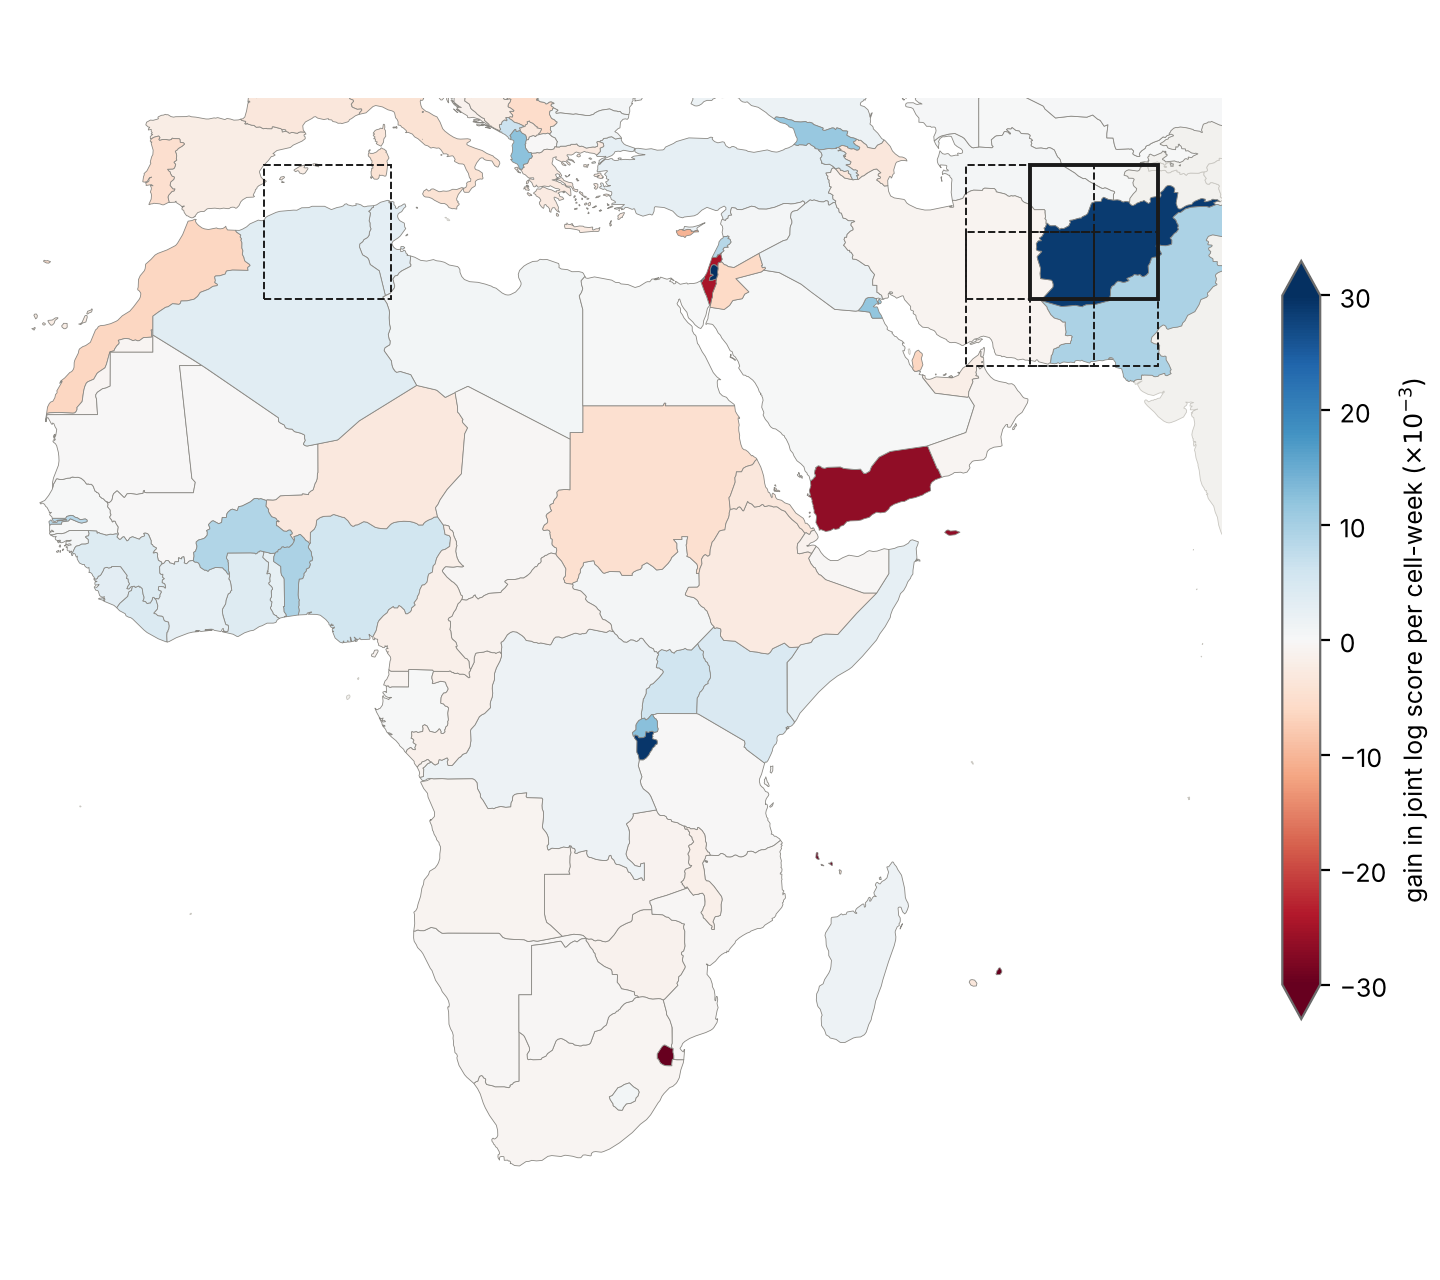
\includegraphics[width=0.85\textwidth]{figures/real_gain_map.png}
\caption{Gain in joint log score per cell-week of the joint model over the product of
the univariate static models, by country, on the 2023--2024 test period (blue: the
joint model predicts better). Boxes: the five $10^\circ \times 10^\circ$ windows with
the largest total gain on the 2022 validation year, selected without the test period;
solid: the first.}\label{fig:gain-map}
\end{figure}

\subsection{The boosting analysis before and after the repair}\label{sec:app-xgb}

Table~\ref{tab:app-xgb} reports three versions of the XGBoost analysis. The first,
\emph{as published}, applies the original procedure to the duplicated table: the
climate variables of the current week and their four-week means as features, positives
weighted by $(n_0/n_1)^{1/2}$, 5 million training rows sampled with replacement, and
the number of trees chosen by early stopping on the test years. The second,
\emph{deduplicated}, applies the same procedure unchanged to the repaired table. It
isolates the effect of the duplication and the leak. The third, \emph{corrected},
also changes the procedure. The number of trees is chosen by early stopping on 2022
after training on 2018--2021, and the model is then refitted on 2018--2022. It uses
no class weight. Its features use only information available before the week, so
the climate variables of the current week are dropped and only their four-week
means are kept. The 5 million training rows are sampled without replacement. The
weighted models are prior-corrected before scoring
(Section~\ref{sec:methods-hybrid}). We also fit the location-aware model of
Section~\ref{sec:methods-diagnostics}, which adds each cell's training event rate to
the corrected model. For the fit that chooses the number of trees, this rate uses
2018--2021 only; for the final fit it leaves out the row's own year.

On the duplicated table we recover the published performance, with AUC-PR 0.934
for conflict and 0.917 for unrest, against 0.93 and 0.91 reported. Split by cell,
nearly all of it comes from the cells that have copies in the original table (AUC-PR
0.966 and 0.968), and in the other cells AUC-PR is 0.498 and 0.528. The first two rows
of Table~\ref{tab:app-xgb} are on different test sets: the duplicated table has
14{,}425{,}130 test rows with conflict prevalence 2.98\%, the repaired table
4{,}787{,}224 rows with 1.62\%. AUC-PR depends on prevalence, so part of the difference
between them is not due to the model. Scored on one row per cell-week of the repaired
test set, the model fitted as published reaches AUC-PR 0.473 for conflict and 0.479
for unrest. The deduplicated and corrected rows are on identical test rows and can be
compared directly. Deduplication alone gives AUC-PR 0.546 for conflict and 0.555 for
unrest. The corrected model reaches 0.544 and 0.557, the persistence baseline 0.481
and 0.468, and the location-aware model 0.566 and 0.583. The scores are similar in
2023 and 2024. On onset rows, where the prevalence is 0.10\% for conflict and 0.14\%
for unrest, the corrected model reaches AUC-PR 0.0073 and 0.0097, and the
location-aware model 0.0111 and 0.0119.

Three conclusions follow. First, a flexible model of history and covariates improves
on persistence, but by less than the published scores suggest: the corrected model
improves on persistence by 0.06 in AUC-PR for conflict and 0.09 for unrest. This gain
cannot be attributed to the covariates alone. The persistence baseline uses only the
total count of the outcome, while the corrected model also uses the five event types
separately, including those of the other outcome, in a nonlinear way, together with
calendar indicators and country-year indicators whose joint values can identify a
country. Second, a cell intercept adds a
further 0.02 to 0.03, so part of what the covariates leave unexplained is persistent
and local. Third, on onset rows all models rank cell-weeks several times better than
chance, but their AUC-PR stays near 0.01. New events in places without recent events
are rarely anticipated.

\begin{table}
\caption{XGBoost on the 2023--2024 test period. As published: duplicated table,
original procedure (current-week features, class weight, early stopping on the test
years). Deduplicated: repaired table, original procedure. Corrected: repaired table,
features available before the week, no class weight, early stopping on 2022.
Corrected + cell event rate: the location-aware model. AUC-PR is also reported
separately for cells that have copies in the original table and for the others.
The persistence baseline ranks cell-weeks by the number of events in the previous four
weeks. The as-published rows are on a different test set from the other rows, with
a different prevalence.}\label{tab:app-xgb}
\centering\small
% Generated by paper/make_real_figures.py; do not edit by hand.
% Inputs (sha256 prefix):
%   results_real/xgb/metrics_corrected_Conflict.json  8fb209c4452d
%   results_real/xgb/metrics_corrected_Unrest.json  17d551c67437
%   results_real/xgb/metrics_corrected_te_Conflict.json  4342ad67c6f3
%   results_real/xgb/metrics_corrected_te_Unrest.json  c27a32300605
%   results_real/xgb/metrics_dedup_Conflict.json  046b10c52ba8
%   results_real/xgb/metrics_dedup_Unrest.json  5370f7674a41
%   results_real/xgb/metrics_original_Conflict.json  37a6e6e5b933
%   results_real/xgb/metrics_original_Unrest.json  9c4718f1c2d2
\begin{tabular}{@{}llrrrcccc@{}}
\toprule
Pipeline & Outcome & Test rows & Prevalence & Trees & AUC-PR & \multicolumn{2}{c}{AUC-PR by cell} & Persistence \\
\cmidrule(lr){7-8}
 & & & & & & dup.\ in original & other cells & AUC-PR \\
\midrule
As published & Conflict & 14.43M & 2.98\% & 1998 & 0.934 & 0.966 & 0.498 & 0.882 \\
As published & Unrest & 14.43M & 3.58\% & 1474 & 0.917 & 0.968 & 0.528 & 0.843 \\
\addlinespace
Original procedure, repaired table & Conflict & 4.79M & 1.62\% & 488 & 0.546 & 0.590 & 0.523 & 0.481 \\
Original procedure, repaired table & Unrest & 4.79M & 2.73\% & 646 & 0.555 & 0.543 & 0.558 & 0.468 \\
\addlinespace
Corrected & Conflict & 4.79M & 1.62\% & 637 & 0.544 & 0.588 & 0.521 & 0.481 \\
Corrected & Unrest & 4.79M & 2.73\% & 814 & 0.557 & 0.545 & 0.559 & 0.468 \\
\addlinespace
Corrected + cell event rate & Conflict & 4.79M & 1.62\% & 381 & 0.566 & 0.598 & 0.549 & 0.481 \\
Corrected + cell event rate & Unrest & 4.79M & 2.73\% & 135 & 0.583 & 0.567 & 0.586 & 0.468 \\
\bottomrule
\end{tabular}

\end{table}

\subsection{Residual spatial structure and the hybrid model}\label{sec:app-hybrid}

We fit the hybrid model~\eqref{eq:hybrid} to the AME region, that is Africa, the
Middle East and adjacent regions (longitude $20^\circ$W to $65^\circ$E, latitude
$36^\circ$S to $45^\circ$N; 13{,}719 cells in 93 countries, 4{,}976{,}634 cell-weeks of
which 1{,}426{,}776 are in the test period; Section~\ref{sec:data-acled}). It
combines the XGBoost offset cross-fitted by country, country effects, and either a
Mat\'ern field with sea barriers (Remark~\ref{rem:boundary}) or independent cell
effects. The offset is trained on the rows of this region only, whereas the corrected
XGBoost model of Section~\ref{sec:app-xgb} is trained on all locations worldwide.
The comparisons below are on identical test rows, but the training sets differ.

Table~\ref{tab:app-diag} reports the test-period residual diagnostics of
every model, and Figure~\ref{fig:app-variogram} the semivariograms of the
test-period residuals. The residuals of the corrected XGBoost model have Moran's $I$
of 0.42 for conflict and 0.15 for unrest (Section~\ref{sec:data-eda}). The
location-aware model reduces it to 0.29 for conflict but increases it to 0.25 for
unrest. The hybrid models do not reduce the overall test-period residual structure. For
conflict, Moran's $I$ is 0.45 with the field or with independent cell effects, about
the same as for the corrected model. For unrest it is 0.29, about twice the value of
the corrected model and above the 0.26 of the cross-fitted offset alone. For unrest,
latent effects estimated on the training years therefore increase the test-period
residual autocorrelation. One possible explanation is that cell effects estimated in
2018--2022 are carried into a period in which recorded unrest rose and its cell-level
pattern changed (Section~\ref{sec:data-acled}); the location-aware model shows a
similar increase. The hybrid models do reduce the residual correlation across borders,
from 0.21 to 0.14 for conflict and from 0.08 to $-0.02$ for unrest. Residual structure
in the test period is therefore not removed by latent effects estimated on the
training years. Section~\ref{sec:app-forecast} examines why. For the cross-fitted
offset, the across-border correlation is 0.25 for pairs of countries in the same fold
and 0.28 for pairs in different folds for conflict, and 0.14 and 0.09 for unrest.
The same-fold pairs are few (264 of 2{,}040).

Table~\ref{tab:app-field} gives the fitted hyperparameters. For
conflict, the field has range 263\,km and standard deviation 1.48. For unrest, the
range is 65\,km and the standard deviation 1.25. A range close to the size of a cell,
about 55~km at the equator, means that the field is not resolved by the grid
(Section~\ref{sec:methods-spde}). The field then behaves like independent cell
effects, and it should not be read as regional hotspots that cross borders. This is
the case for unrest. The field improves the log marginal likelihood over independent
cell effects by 1{,}254 for conflict but only by 95 for unrest, and the two give almost
the same test scores for unrest (Table~\ref{tab:app-forecast}). For unrest,
cell-level effects would largely track towns and cities, where protests are both more
frequent and more often reported. A fit to all locations worldwide (46{,}031 cells)
gives a range of 313\,km for conflict and 65\,km for unrest. The unrest results of the
AME region also depend on its composition. It includes Mediterranean Europe, where
unrest is dense and where several countries enter ACLED only in 2020
(Section~\ref{sec:data-acled}). The univariate analyses of this section use that
earlier region; the joint analyses of the main text exclude the countries of Europe,
and we have not repeated the univariate analyses on the restricted region.

Figure~\ref{fig:app-fitted} compares observed and predicted frequencies over the
test period. The hybrid model reproduces the regional pattern of both outcomes,
including the Sahel, eastern Congo, Somalia, Yemen and Syria--Iraq for conflict.
For both outcomes the hybrid model is close to the diagonal above a predicted
probability of about 1\% and overpredicts below it, where the observed frequency is
lower than predicted. The cross-fitted offset alone underpredicts in the same bins.

\begin{figure}
\centering
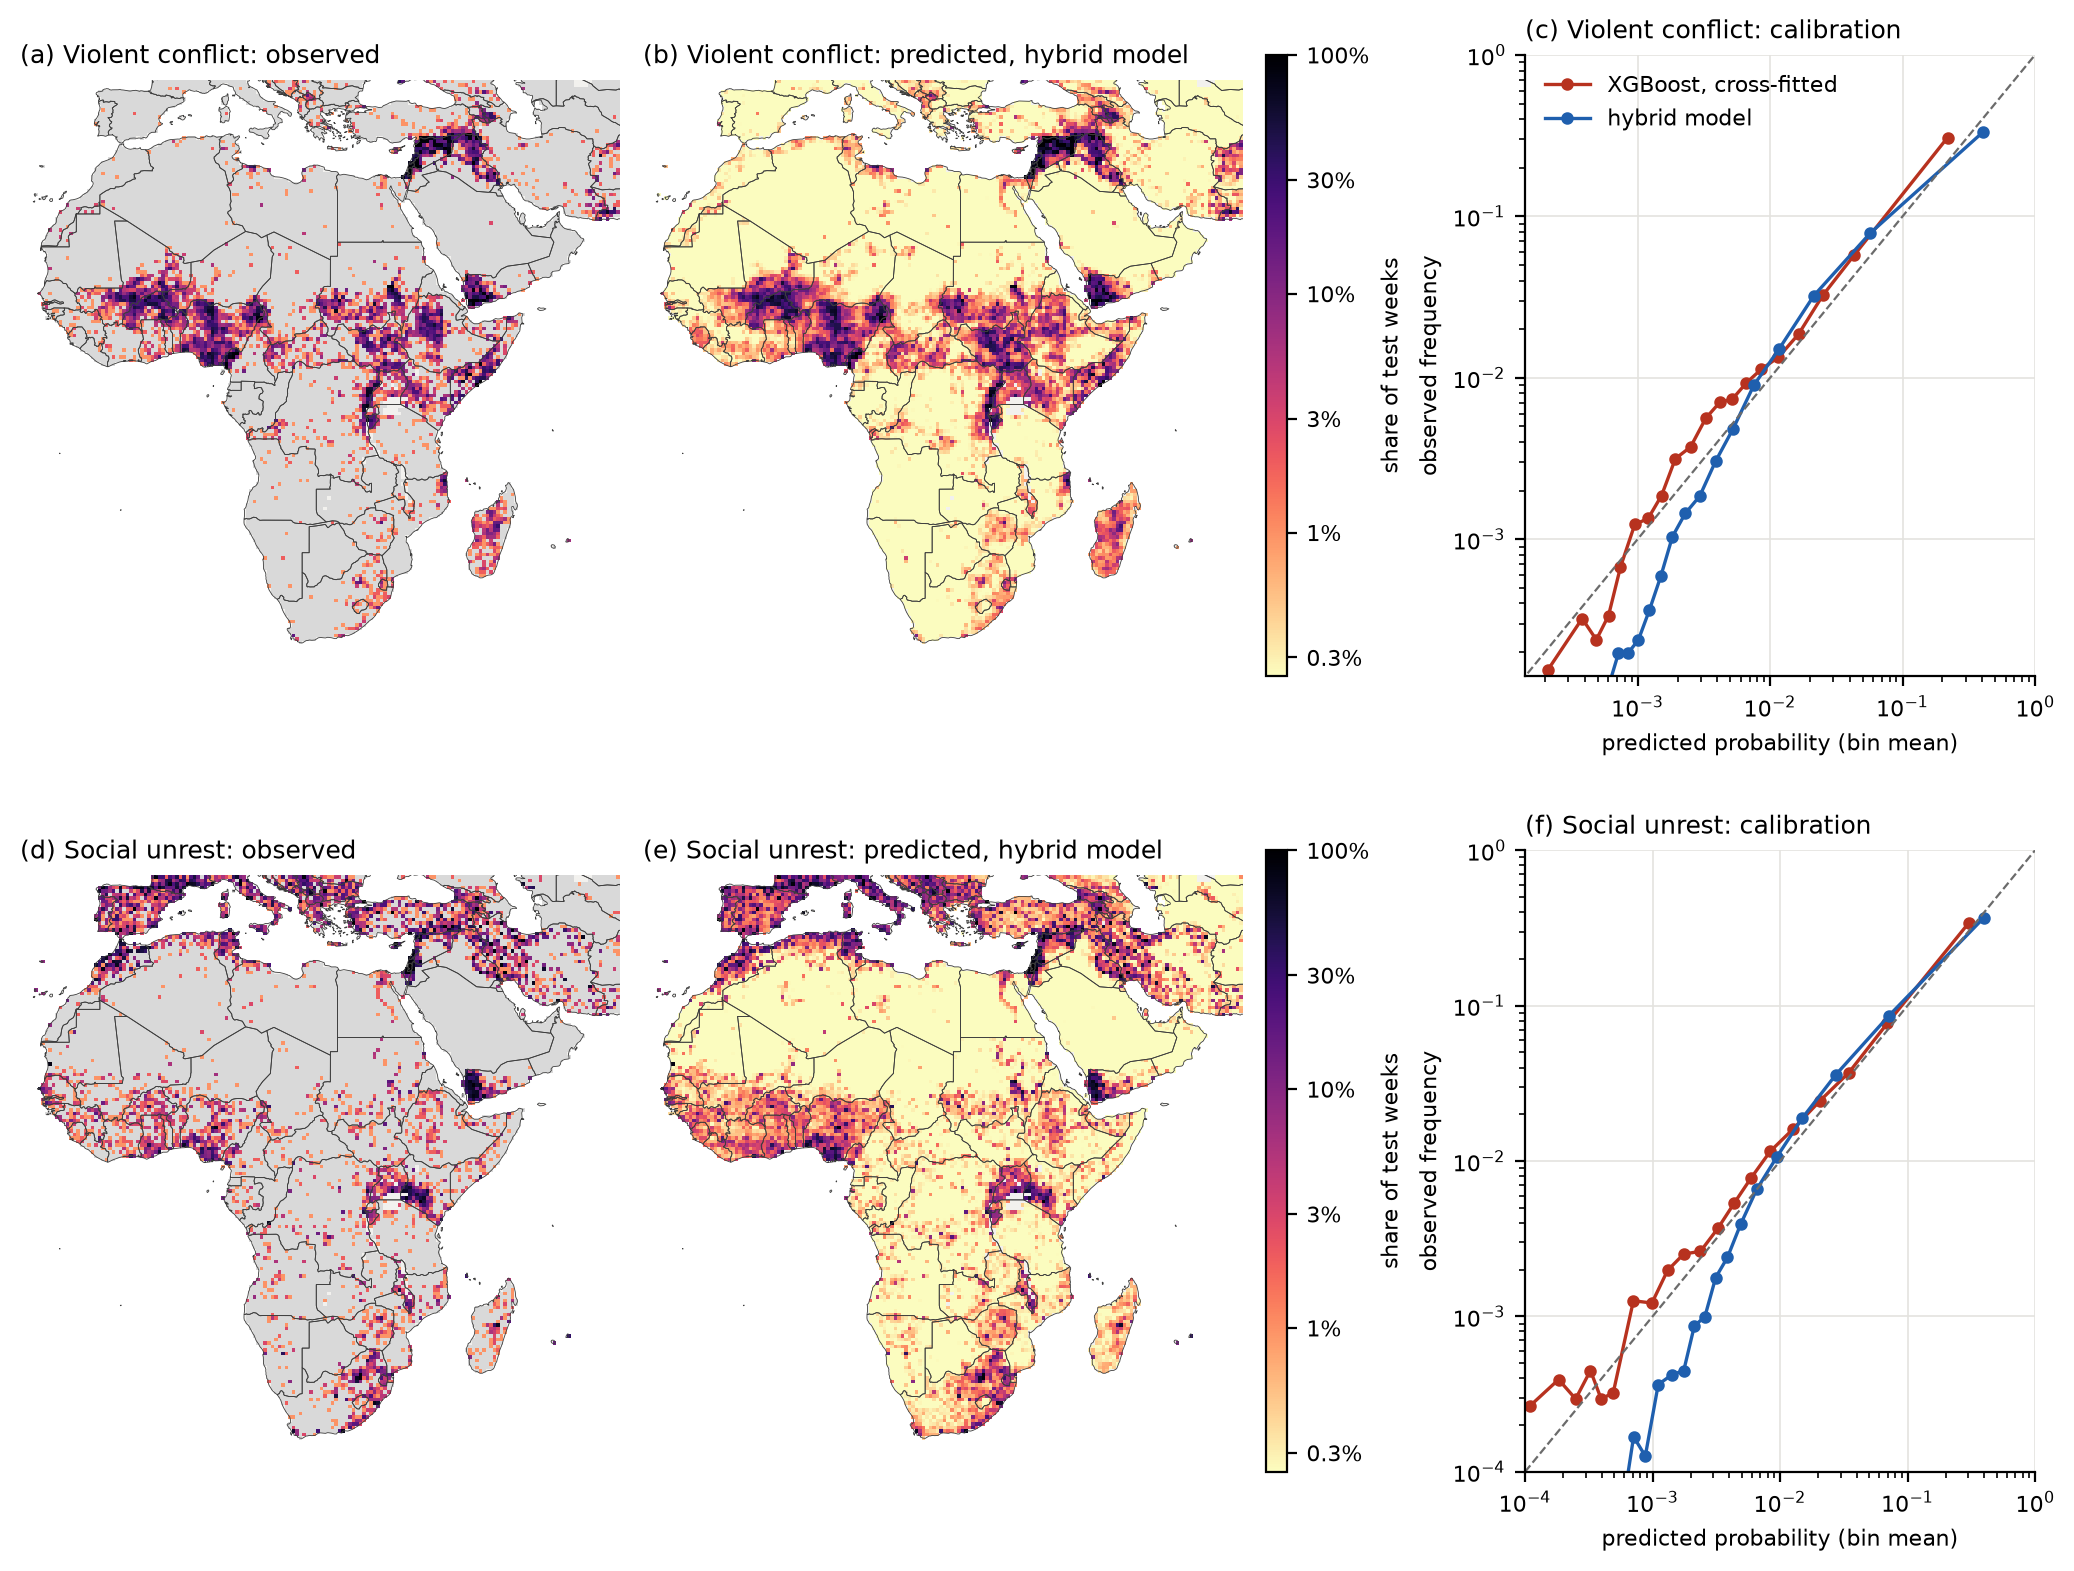
\includegraphics[width=\textwidth]{figures/real_fitted.png}
\caption{Observed and predicted event frequency in the test period 2023--2024,
AME region. (a, d) Share of test weeks with at least one event in each
cell; grey cells have no event week. (b, e) Mean predicted probability of the hybrid
model with country effects and the Mat\'ern field over the same weeks, on the same
colour scale. (c, f) Calibration: observed frequency against mean predicted probability
in 20 equal-count bins, for the hybrid model and the XGBoost offset cross-fitted by
country; the dashed line is perfect calibration.}\label{fig:app-fitted}
\end{figure}

The estimated fields are shown in Figure~\ref{fig:app-field}.
Table~\ref{tab:app-boxes} summarises the posterior of the field averaged
over eleven regions. The regions were chosen before the fit: eight known conflict
zones and three regions expected to be quiet. A posterior probability close to one
that the average over a known conflict zone is positive is therefore expected and is
not a finding in itself. The last two rows of the table give a summary that does not
depend on chosen regions: the share of cells whose posterior probability that
$w(s) > 0$ exceeds 0.95, and the share for which it is below 0.05. For conflict these
shares are 18.9\% and 3.0\%, and for unrest 11.6\% and 2.6\%. For conflict, the
averages over the three quiet regions, the western Congo basin, the interior of the
Arabian peninsula and southern Africa, are negative. For unrest, only the average
over eastern Congo is clearly positive, and none is clearly negative. Negative
values of $w$ mark low \emph{recorded} risk relative to the covariates, recent history
and country effects. In regions with restricted media access and few ACLED sources,
such as the interior of the Arabian peninsula, they may reflect reporting rather than
occurrence (Section~\ref{sec:data-acled}). Positive values in cells with towns or
administrative centres may in part reflect events of low spatial precision, which
ACLED places at such centroids. Because the offset is cross-fitted by country, errors
of the offset that are common to a country are absorbed by $u$, but errors that vary
within a country can be absorbed by $w$.

\begin{figure}
\centering
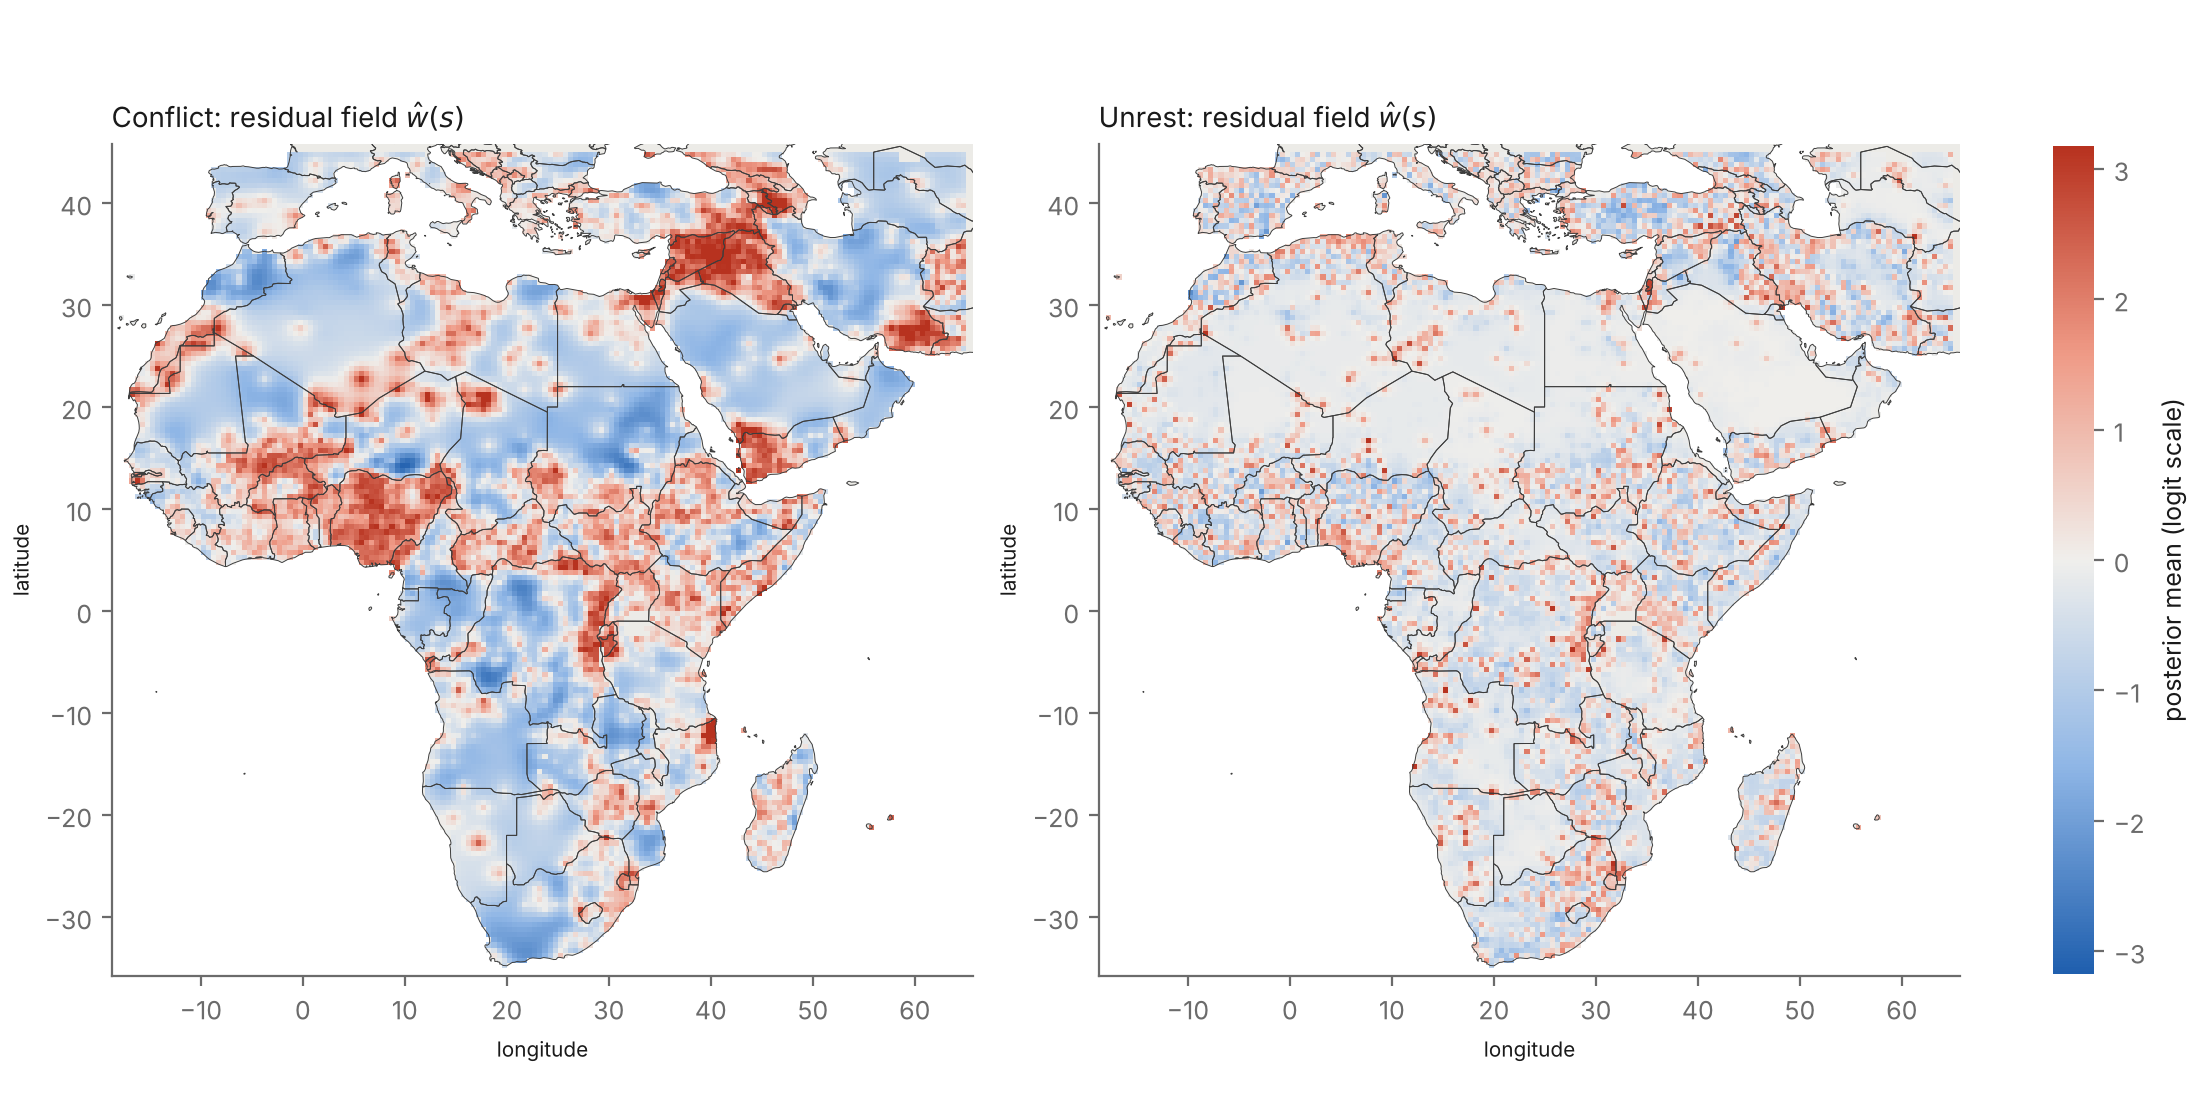
\includegraphics[width=\textwidth]{figures/real_field.png}
\caption{Posterior mean of the residual field $w(s)$ of the hybrid model for conflict
(left) and unrest (right), on the logit scale. Positive values mark higher recorded
risk than predicted by the covariates, recent event history and country effects.
Recorded risk mixes occurrence and reporting, and events of low spatial precision are
placed at town and administrative centroids (Section~\ref{sec:data-acled}).}\label{fig:app-field}
\end{figure}

\subsection{Forecasting}\label{sec:app-forecast}

Table~\ref{tab:app-forecast} compares out-of-sample scores on identical test rows of
the AME region. The reference is the corrected XGBoost model. Differences
in mean log score are given against it, with standard errors clustered by country
(standard errors clustered by cell are smaller). A gain of a hybrid model over the
cross-fitted offset alone is not evidence for the latent effects
(Section~\ref{sec:methods-hybrid}). The relevant comparisons are with the corrected
and location-aware models. The table has two parts. In the static part, every model
is fitted once on 2018--2022. In the updated part, the models are updated each
quarter of the test period with all data before the start of the quarter, as an
early-warning system would be run. The location-aware boosting model is updated by
recomputing the cell event rate. The hybrid models keep the hyperparameters fitted on
2018--2022 and recompute the latent effects. Table~\ref{tab:app-dynamic}
reports all dynamic experiments.

\paragraph{Static models.} With the field, the hybrid model improves on the corrected
XGBoost model in log score by 0.0021 (SE 0.0007) for unrest. For conflict the
difference, 0.0012 (SE 0.0009), is within about one standard error. The hybrid models
do not reach the location-aware model, which improves on the corrected model by
0.0035 (SE 0.0013) and 0.0032 (SE 0.0008). The Brier score, which
Table~\ref{tab:app-forecast} does not report, points the other way for conflict. The
hybrid model with the field has a Brier score higher than the corrected model by
0.0004 (SE 0.0002) for conflict, and lower by 0.0001 (SE 0.0002) for unrest. The
location-aware model lowers the Brier score by 0.0003 (SE 0.0002) and 0.0004
(SE 0.0002). The field and the independent cell effects
give almost the same scores: for conflict the field is better by 0.0002 in log score,
and for unrest by less than 0.0001. A hybrid model with a space-time field
($\Delta = 13$ weeks, forecast through its AR(1) dynamics) improves only slightly on
the static field, by 0.0004 for conflict and 0.0003 for unrest. In AUC-PR, the
corrected model reaches 0.515 for conflict and 0.532 for unrest, the hybrid model with
the field 0.519 and 0.540, the location-aware model 0.533 and 0.550, and persistence
0.446 and 0.451. On onset rows, where the prevalence is 0.15\% for conflict and 0.18\%
for unrest, AUC-PR is 0.008 to 0.011 for conflict and 0.010 to 0.014 for unrest for all
models except the cross-fitted offset alone, which reaches 0.006 and 0.009.

\paragraph{Updated models.} Quarterly updating improves every model that is updated;
the corrected XGBoost model and the cross-fitted offset are not updated. The updated
hybrid model with the space-time field improves on the corrected XGBoost model by
0.0035 (SE 0.0008) for conflict and 0.0034 (SE 0.0007) for unrest. It thus reaches the
score of the static location-aware model, and its AUC-PR is 0.539 and 0.554. It also
has the highest AUC-PR on onset rows, 0.0120 for conflict and 0.0142 for unrest.
Updating also improves the location-aware model, however, to 0.0050 (SE 0.0013) and
0.0044 (SE 0.0008) in log score, and AUC-PR 0.544 and 0.559. Of the gap in log score
between the static hybrid model with the field and the static location-aware model,
0.0023 for conflict and 0.0012 for unrest, a gap of 0.0015 and 0.0010 remains between
the best updated models of each kind. In the Brier score the updated space-time hybrid
model is better than the corrected model, by 0.0001 (SE 0.0001) for conflict and
0.0004 (SE 0.0002) for unrest, and the updated location-aware model by 0.0005
(SE 0.0002) and 0.0006 (SE 0.0002). The updated space-time hybrid model removes most
of the test-period residual structure: Moran's $I$ of its residuals is 0.12 for
conflict and 0.10 for unrest, against 0.32 and 0.26 for the updated location-aware
model.

We also refitted the hybrid models, including the boosting offset and the
hyperparameters, on 2018--2023 and scored 2024. These comparisons are on the 2024 rows
only. The refitted hybrid model with the field improves on the corrected model by
0.0022 for conflict and 0.0033 for unrest, against 0.0007 and 0.0017 without the
refit. The location-aware model, which is not refitted in this experiment, improves on
it by 0.0028 and 0.0023. A year of new data thus brings the hybrid model close to the
location-aware model for conflict and ahead of the static location-aware model for
unrest.

\paragraph{Where the residual structure lies.} To see why latent effects estimated on
the training years help little, we fitted the field and the independent cell effects
to the test period itself, with the same offset. This is an in-sample upper bound on
what a static latent term can absorb. For conflict, the test-period field has a range
of 374\,km, the field fits much better than independent cell effects (log marginal
likelihood higher by 1{,}045), and it removes the residual autocorrelation (Moran's $I$
from 0.54 to $-0.12$, against 0.35 with independent cell effects). Its correlation
with the field fitted on 2018--2022 is 0.79. For unrest, the test-period field has a
range of 66\,km, its advantage over independent cell effects is small (69 in log
marginal likelihood), and its correlation with the training field is 0.69. Conflict
residual risk is therefore smooth at a scale of a few hundred kilometres and partly
moves over time, which is why updating, and a space-time field, help. Unrest residual
risk is mainly cell-level, which is what a cell event rate captures directly. A
location-aware boosting model is a strong benchmark for both.

\begin{table}
\caption{Out-of-sample scores, AME region, 2023--2024, on identical
test rows. Static models are fitted once on 2018--2022; updated models are updated
each quarter with all data before the quarter (hybrid models: latent effects
recomputed with the hyperparameters fixed; location-aware model: cell event rate
recomputed). Differences in mean log score against the corrected XGBoost model, with
standard errors clustered by country. Lower is better for the log score. The hybrid
offset is trained on the AME region only; the corrected and
location-aware XGBoost models are trained on all locations. Onset rows: cells without
an event of the outcome in the previous 52 weeks. Further experiments in Table~\ref{tab:app-dynamic}.}\label{tab:app-forecast}
\centering\small
% Generated by paper/make_real_figures.py; do not edit by hand.
% Inputs (sha256 prefix):
%   results_real/compare/compare_conflict.json  f9cfaa08c2c7
%   results_real/compare/compare_conflict_st.json  41eadb9f67f6
%   results_real/compare/compare_conflict_update.json  e016ec0c6b38
%   results_real/compare/compare_unrest.json  b8e39ca9067c
%   results_real/compare/compare_unrest_st.json  8d037dd2f5c8
%   results_real/compare/compare_unrest_update.json  4c3deb048ccd
\resizebox{\textwidth}{!}{%
\begin{tabular}{@{}lcccccc@{}}
\toprule
Model & \multicolumn{3}{c}{Conflict} & \multicolumn{3}{c}{Unrest} \\
\cmidrule(lr){2-4}\cmidrule(lr){5-7}
 & AUC-PR & $\Delta$ log score & $\Delta$ Brier & AUC-PR & $\Delta$ log score & $\Delta$ Brier \\
 & & $\times 10^3$ (SE) & $\times 10^3$ (SE) & & $\times 10^3$ (SE) & $\times 10^3$ (SE) \\
\midrule
\multicolumn{7}{@{}l}{\emph{Fitted once on 2018--2022}} \\
\quad XGBoost, corrected (reference) & 0.515 & reference & reference & 0.532 & reference & reference \\
\quad XGBoost + cell event rate & 0.533 & $-3.50$ (1.27) & $-0.32$ (0.22) & 0.550 & $-3.22$ (0.78) & $-0.36$ (0.18) \\
\quad XGBoost, cross-fitted by country (offset) & 0.461 & $8.24$ (2.27) & $1.39$ (0.42) & 0.493 & $4.74$ (1.20) & $0.91$ (0.28) \\
\quad Offset + $u$ + iid cell effects & 0.519 & $-0.93$ (0.89) & $0.42$ (0.21) & 0.540 & $-2.04$ (0.67) & $-0.10$ (0.18) \\
\quad Offset + $u + w$ & 0.519 & $-1.17$ (0.94) & $0.44$ (0.23) & 0.540 & $-2.07$ (0.66) & $-0.10$ (0.18) \\
\quad Offset + $u$ + cell effects + $v$, 13-week steps & 0.519 & $-1.56$ (0.96) & $0.30$ (0.24) & 0.541 & $-2.33$ (0.79) & $-0.19$ (0.21) \\
\quad Offset + $u$ + cell effects + $v$, 26-week steps & 0.518 & $-1.52$ (0.95) & $0.34$ (0.25) & 0.540 & $-2.29$ (0.80) & $-0.17$ (0.22) \\
\addlinespace
\multicolumn{7}{@{}l}{\emph{Updated each quarter of the test period}} \\
\quad XGBoost + cell event rate & 0.544 & $-4.98$ (1.31) & $-0.54$ (0.23) & 0.559 & $-4.38$ (0.83) & $-0.59$ (0.17) \\
\quad Offset + $u$ + iid cell effects & 0.531 & $-2.30$ (0.76) & $0.12$ (0.14) & 0.550 & $-3.03$ (0.72) & $-0.35$ (0.18) \\
\quad Offset + $u + w$ & 0.531 & $-2.65$ (0.77) & $0.11$ (0.14) & 0.550 & $-3.06$ (0.72) & $-0.35$ (0.18) \\
\quad Offset + $u$ + cell effects + $v$, 13-week steps & 0.539 & $-3.52$ (0.81) & $-0.14$ (0.09) & 0.554 & $-3.39$ (0.71) & $-0.42$ (0.17) \\
\addlinespace
Persistence (past 4 weeks) & 0.446 & -- & -- & 0.451 & -- & -- \\
\bottomrule
\end{tabular}
}

\end{table}

\subsection{State dependence, climate and national indicators}\label{sec:app-glmm}

The parametric latent models of Section~\ref{sec:methods-model} are fitted to the AME
region (3{,}494{,}982 training rows, 13{,}719 cells). We compare
logistic regression without latent effects, a model with country effects, and models
with country effects, independent cell effects and a Mat\'ern field, with and without
a spatially varying coefficient for maximum temperature and with the spatial+
adjustment of Section~\ref{sec:methods-confounding}.

\paragraph{State dependence.} The coefficient $\delta$ of the own four-week history is
2.04 (SE 0.007) for conflict in logistic regression, 1.75 with country effects and
0.92 (SE 0.008) with country effects, cell effects and the field. For unrest it is
1.62, 1.47 and 0.78. The coefficient of the other outcome's history falls in the same
way, from 0.40 to 0.15 for unrest on conflict and from 0.22 to 0.13 for conflict on
unrest. In the central Sahel ($9^\circ$N to $20^\circ$N, $6^\circ$W to $16^\circ$E, a
box of $22^\circ$ by $11^\circ$; 968 cells, steps of 8 weeks), adding a space-time field
lowers $\hat\delta$ further: for conflict from 1.58 without latent effects to 0.65
with the static terms and 0.28 (SE 0.021) with the space-time field, whose range is
230\,km and AR(1) coefficient 0.93 per 8 weeks. For unrest the corresponding values
are 1.27, 0.42 and 0.17 (SE 0.060), with an AR(1) coefficient of 0.49 per 8 weeks,
about 0.915 per week. Much of the apparent state dependence is therefore absorbed by
latent risk that varies slowly in space and time. Three caveats apply. First, the
central Sahel models have no neighbour histories, so a space-time field at this scale
can also absorb diffusion of events between neighbouring cells. In West Africa,
adding the space-time field lowers the coefficient of conflict in neighbouring cells
from 0.129 (SE 0.007) to 0.051 (SE 0.008) (Table~\ref{tab:app-joint}). The fall in
$\hat\delta$ therefore cannot distinguish persistent latent risk from spatio-temporal
diffusion. Second, in S3 the empirical SD of $\hat\delta$ was 1.19 to 1.66 times its
mean SE whenever a space-time field was fitted, so the SEs above are too small,
by an amount that varies across settings. Third, the unrest dynamics are in the regime
of S3 ($\phi$ about 0.9 per week, $\Delta = 8$) in which $\hat\delta$ kept an upward
bias of about 0.10 under pure heterogeneity. The field $v$ is also defined on the
observed cells only, with reflecting edges, which departs from Remark~\ref{rem:boundary};
in the space-time hybrid models the same holds for the static part. $\hat\delta$ under
$v$ should be read with that caveat. As in S3 (Section~\ref{sec:sim-persistence}), we
read the remaining $\hat\delta$ as conditional dependence of recorded events
(Section~\ref{sec:methods-persistence}), not as contagion.

\paragraph{Climate.} All models condition on the event histories of the previous four
weeks and on the latent effects. The climate coefficients are therefore short-run
direct associations. Any effect of climate that acts through earlier events is
blocked, and we do not estimate total effects. In the model with the field, the
coefficients of the five standardised anomalies for conflict are 0.015 (SE 0.006) for
maximum temperature, $-0.007$ (SE 0.006) for minimum temperature, $-0.003$ (SE 0.005)
for precipitation, $-0.004$ (SE 0.004) for drought and 0.005 (SE 0.007) for
PM$_{2.5}$. For unrest they are 0.009 (SE 0.007), $-0.021$ (SE 0.006), $-0.017$
(SE 0.005), $-0.006$ (SE 0.004) and 0.033 (SE 0.007). The unrest coefficients of
minimum temperature and precipitation are thus 3 to 4 SE from zero and larger in
absolute value than that of maximum temperature. These SEs treat cell-weeks as
conditionally independent given the static latent effects, and residual space-time
dependence would make them too small, so we do not read the conflict coefficient of
maximum temperature, 2.5 SE from zero, as clear evidence. The PM$_{2.5}$ anomaly is
not interpretable. PM$_{2.5}$ is missing in 55.5\% of training rows and its
climatological standard deviation is undefined in 91{,}392 of the 164{,}628
cell-months, so the floor is about $10^{-9}$ and standardised anomalies can be
extreme (Section~\ref{sec:data-cov}). Of the five, we examine the maximum-temperature
anomaly in more detail. The biome-specific slopes of the model with a spatially varying coefficient lie
between $-0.16$ and $0.08$ for conflict and between $-0.09$ and $0.06$ for unrest, and
none is more than two standard errors from zero. The spatially varying part has
standard deviation 0.076 for conflict and 0.072 for unrest, so variation within biomes
is negligible, and the model does not improve the marginal likelihood or the test
scores over the model without it. Conditional on recent event history and the latent
effects, the short-run direct association of maximum-temperature anomalies with the
weekly probability of recorded events is therefore small in the AME region, and we find
no evidence that it differs between or within biomes. This statement does not extend
to the other anomalies, nor to total effects of climate.

\paragraph{National indicators.} Without latent effects, several between-country
coefficients are large and estimated with standard errors below 0.02, for example
$-0.56$ (SE 0.008) for the EPI on conflict and 0.12 (SE 0.005) for the liberal
democracy index on unrest. With country effects their standard errors grow by an order
of magnitude, and with the field they change further: $-0.22$ (SE 0.12) for the EPI on
conflict and 0.21 (SE 0.14) for the liberal democracy index on unrest. They are also
unstable under spatial+: for the EPI on conflict $-0.23$, $-0.22$ and $-0.07$ with
$m = 10$, 20 and $m^* = 138$, and for the liberal democracy index on unrest 0.17, 0.20
and $-0.02$ with $m = 10$, 20 and $m^* = 176$. In the light of S2
(Section~\ref{sec:sim-confounding}), the between-country coefficients cannot be
separated from spatially smooth unmeasured risk, and we do not interpret them.

The within-country coefficients are identified from changes over time within a
country. Across the models with the field (with the field, with the spatially varying
coefficient, and spatial+), they barely change, for example 0.014 to 0.016 for the EPI
on conflict and 0.030 for the liberal democracy index on unrest. They are not all
small. In the model with the field, the within coefficients on conflict are 0.095
(SE 0.007) for log GDP per capita, $-0.082$ (SE 0.011) for greenhouse gas emissions and
0.049 (SE 0.010) for the ecological footprint, several times the
maximum-temperature coefficient. Their standard errors, however, treat cell-weeks as
conditionally independent, whereas the within variation comes from about 93 countries
over five training years. Like the between coefficients, they rest on few independent
contrasts, and their model-based standard errors are too small by an unknown amount.
We therefore do not interpret them either. Access to electricity needs a further
caveat. Unlike the other national indicators, it is not re-attached per country and
year in the repaired table (Section~\ref{sec:data-acled}), so in cells that had copies
it can carry the value of a neighbouring country. Its within component then mixes
change over time with differences across borders. This may explain why its within
coefficient on conflict is $-0.106$ (SE 0.005) without latent effects but $-0.027$
(SE 0.023) with the field, and on unrest 0.008 (SE 0.006) without latent effects but
0.072 (SE 0.024) with the field. We do not interpret the electricity coefficients.

\paragraph{Missingness.} Two missingness indicators were dropped because they are
constant in the training rows (EPI and liberal democracy index), and the material and
ecological footprint indicators were merged with that of greenhouse gas emissions. The
remaining indicators are not interpretable as effects. They vary mostly between
countries, so they are confounded with the country effects and the field, and their
signs change across specifications. For a missing GDP the coefficient on conflict is
0.31 (SE 0.022) without latent effects, $-0.08$ (SE 0.061) with country effects and
$-0.26$ (SE 0.056) with the field. For a missing IPC analysis the coefficient on unrest
is 0.06 (SE 0.020), 0.20 (SE 0.023) and $-0.18$ (SE 0.030) in the same three models.
The other indicators have large standard errors, and we do not interpret any of them.
